\chapter{Motion planning}

This chapter will focus on the motion planning part. You will learn how to select the motion planner you want (RRT, RRT*, STOMP, CHOMP...), how to create a planning problem and how to solve it.

\section{GUI utilisation}

We can directly use the GUI to solve some motion planning problems. Indeed, moveit has an interface in rviz. Using the GUI will be usefull when you want to quickly test your robot motion or a planning problem. It can also show how long it will last for the motion planner you selected to find a motion plan. However, when you will need to find precise plan (with exact coordinate for joints) or when you will want to generate a lot of trajectories it will be far easier to use scripts.


\begin{figure}
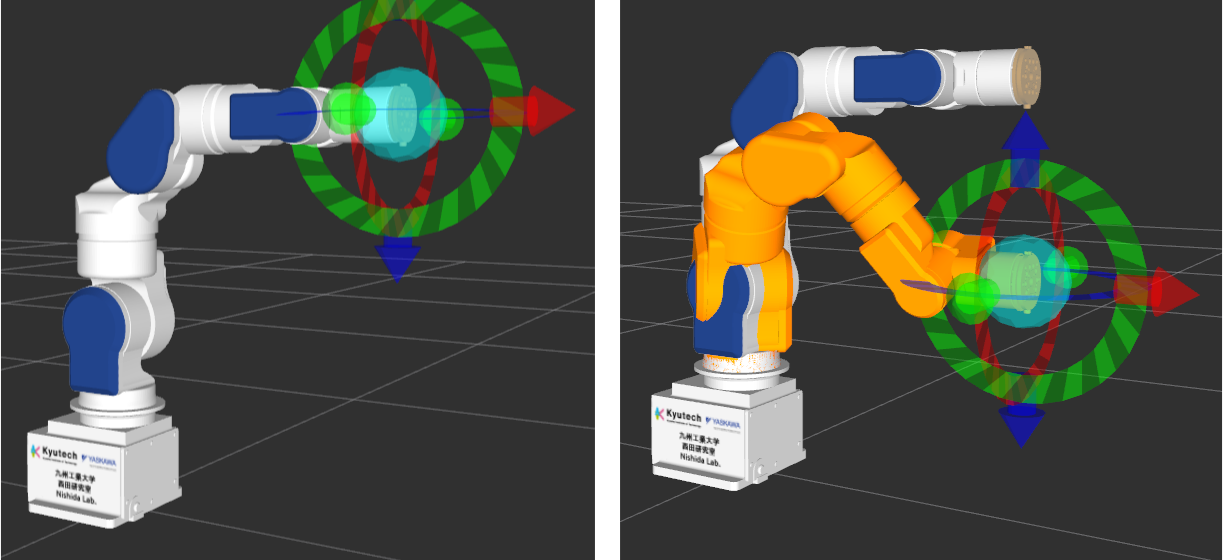
\includegraphics[scale=0.27]{images/motion_planning/gui_end_effector.png}
\centering
\caption{Changing the goal position by moving the end effector ball through the GUI.}
\label{fig:gui_end_effector}
\end{figure}